%---------------------------------------------------------------------
%
%                          Ap�ndice 1
%
%---------------------------------------------------------------------


\chapter{Documentaci�n}
\label{ap1:documentacion}

	\section{Documento de Especificaci�n de Requerimientos}
		\label{ap1:ERS}
		%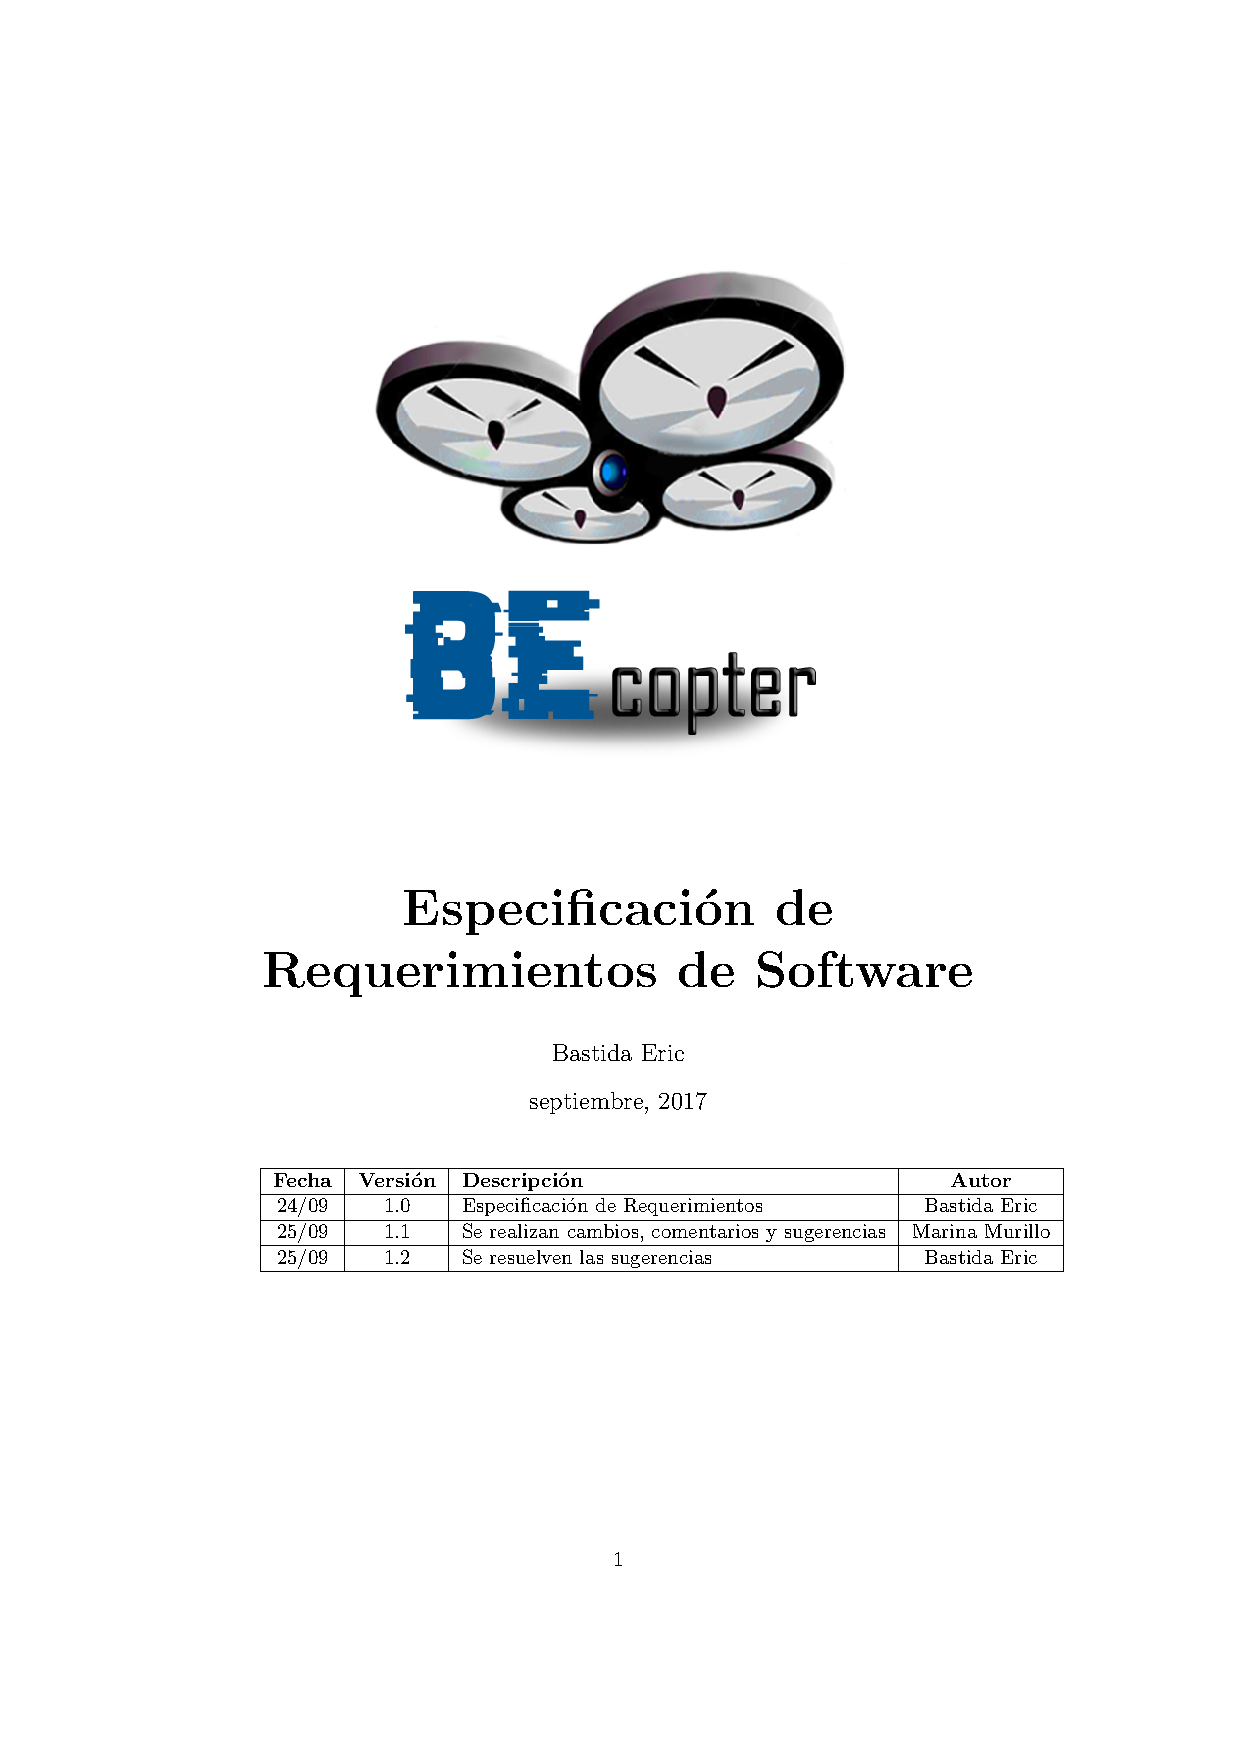
\includepdf[pages=-]{Apendices/Apendice_files/ERS}
		%TODO: Descomentar la linea al momento de entregar el informe. Se comenta en el caso se edicion (m�s r�pido)
		
	\section{Manual de usuario}
		\label{ap1:user_manual}
		%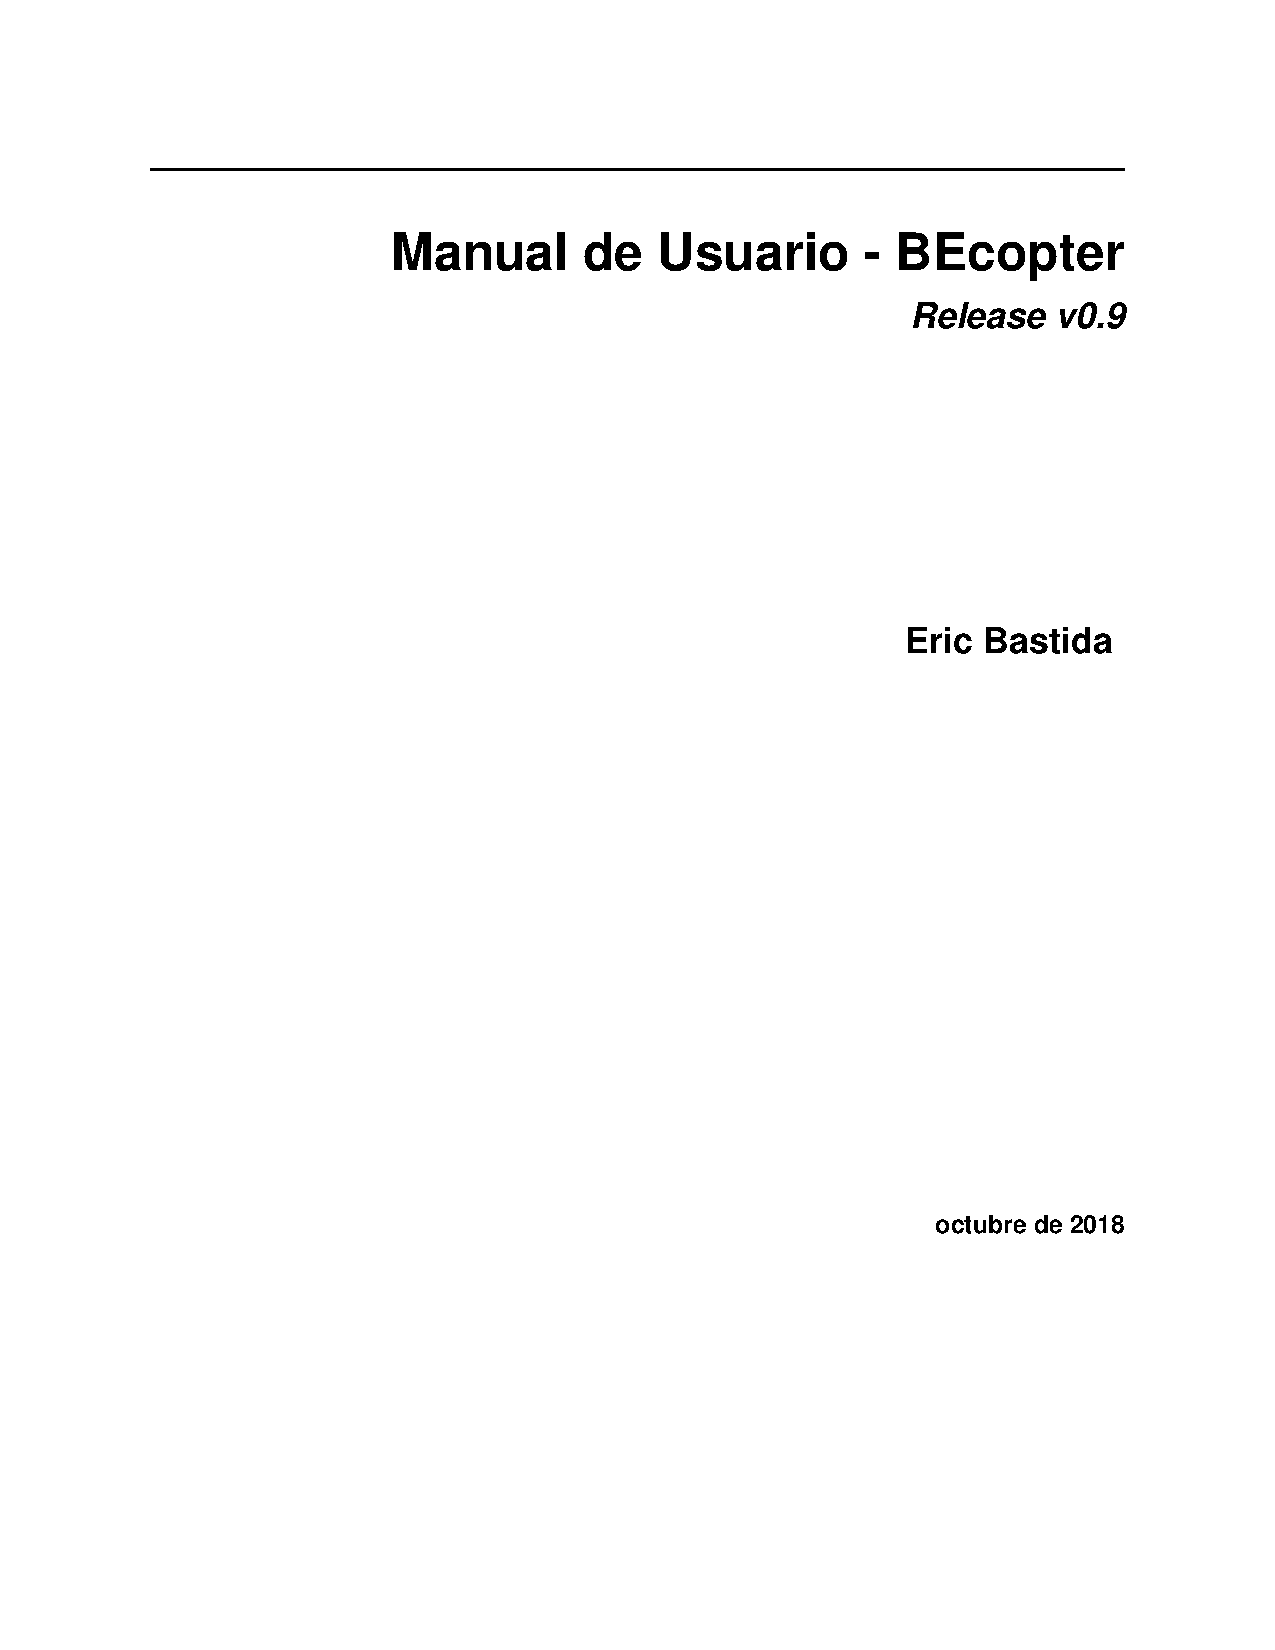
\includepdf[pages=-]{Apendices/Apendice_files/Manual}
		%TODO: Descomentar la linea al momento de entregar el informe. Se comenta en el caso se edicion (m�s r�pido)
	
	\section{Mockups de la interfaz gr�fica del proyecto}
		\label{ap1:mockup}
		%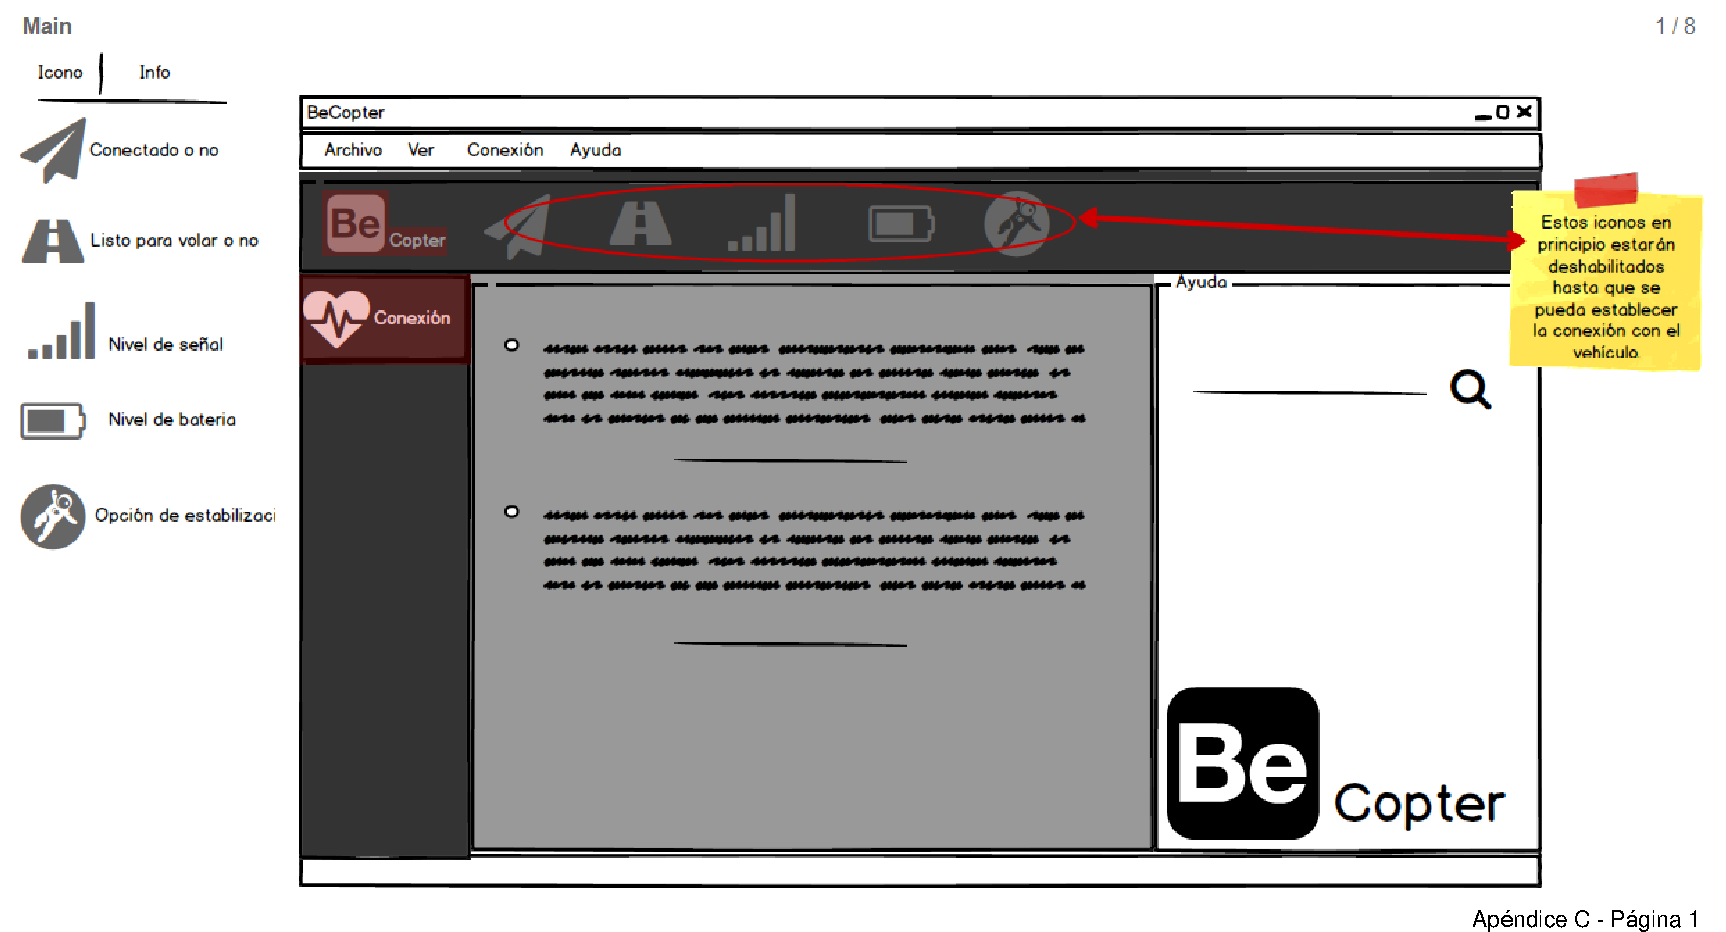
\includepdf[pages=-]{Apendices/Apendice_files/Mockup}
		%TODO: Descomentar la linea al momento de entregar el informe. Se comenta en el caso se edicion (m�s r�pido)
	
	\section{Interfaz Gr�fica del Usuario (GUI)}
		\label{ap1:GUI}
		%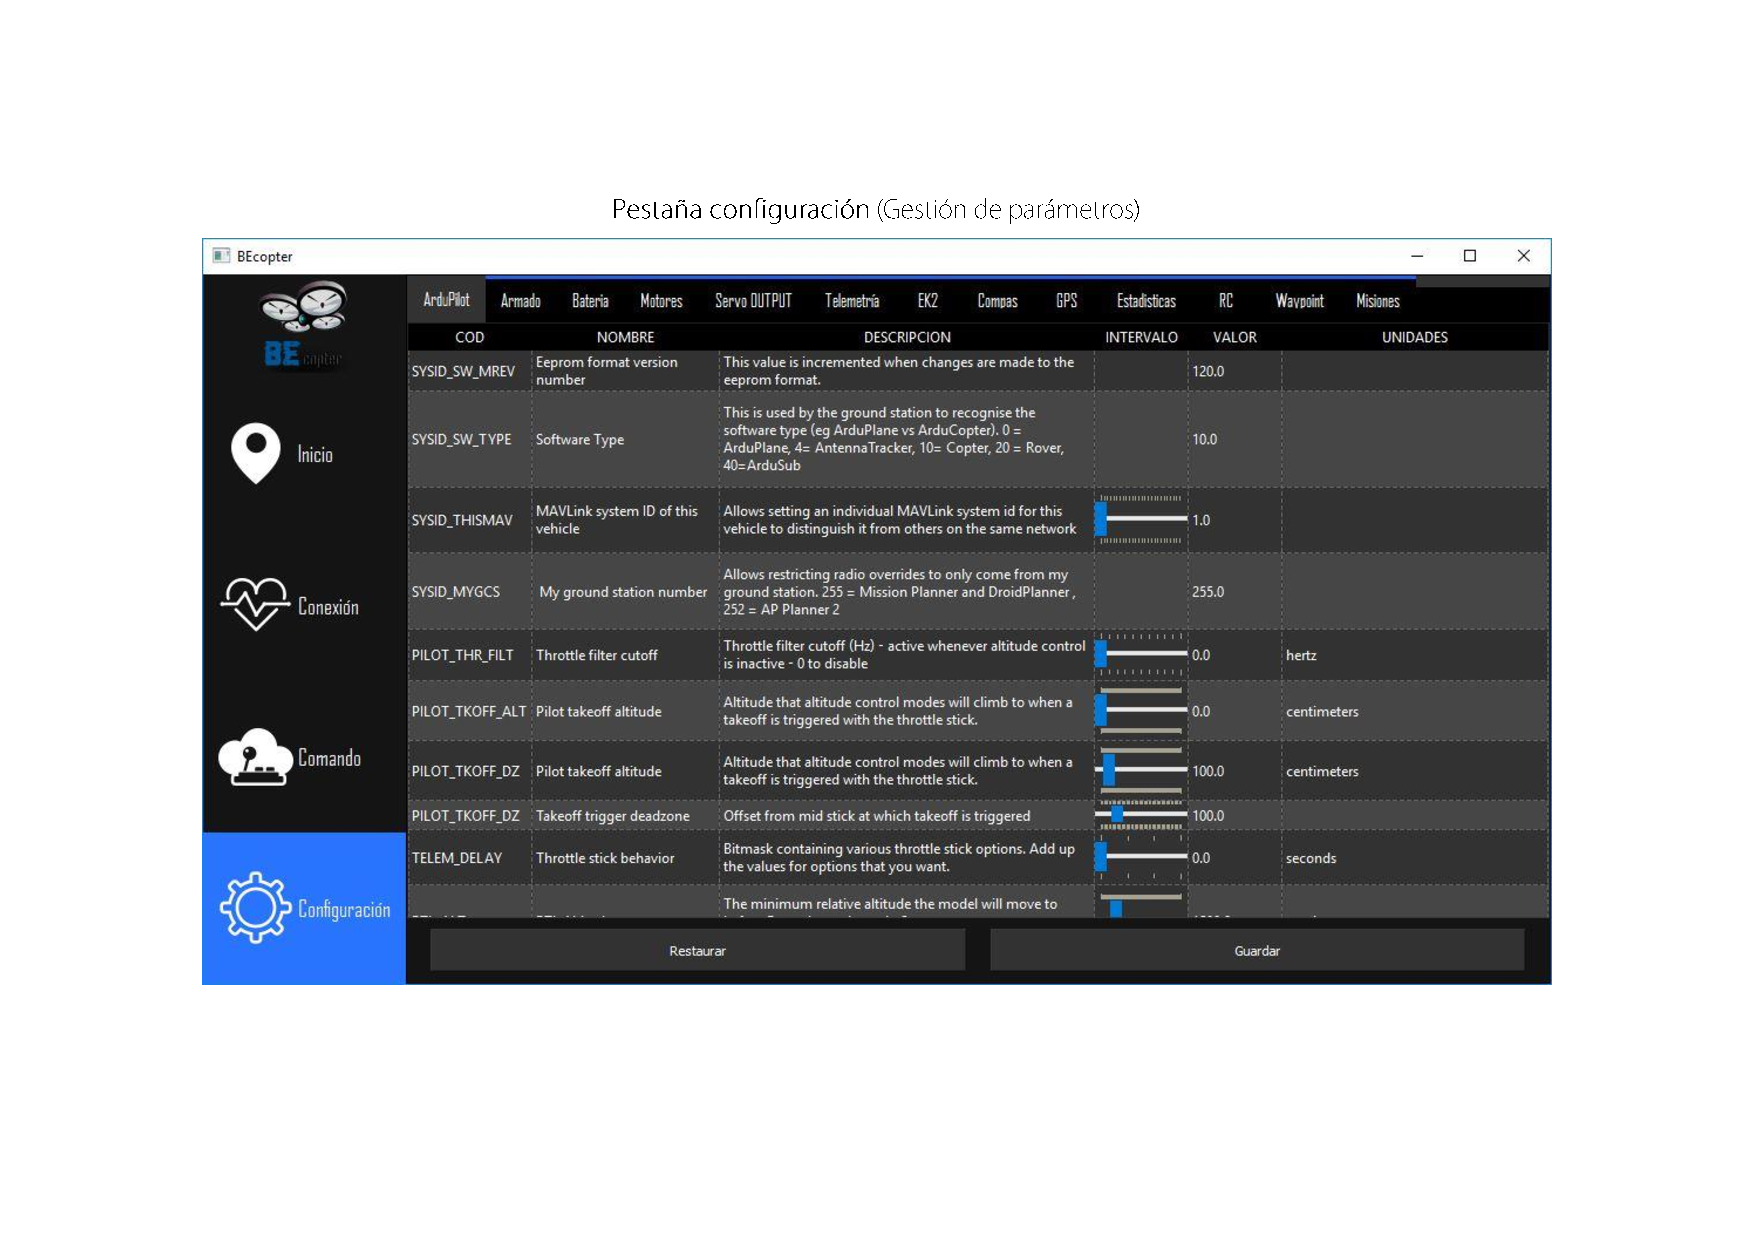
\includepdf[pages=-]{Apendices/Apendice_files/GUI}
		%TODO: Descomentar la linea al momento de entregar el informe. Se comenta en el caso se edicion (m�s r�pido)

	
	\section{Diagrama de clases inicial del Proyecto}
		\label{ap1:classDiagra_v0}
%		\begin{figure}[!h]
%			\centering
%			\includegraphics[scale=0.45, angle=-90width=\linewidth, height=0.93\textheight]Apendice/Apendice_files/ClassDiagram}
%		\end{figure}

%		\caption{Diagrama de clases inicial de BEcopter.}
		%TODO: Descomentar la linea al momento de entregar el informe. Se comenta en el caso se edicion (m�s r�pido)
		
	\section{Diagrama de clases final del Proyecto}
	\label{ap1:classDiagra_vFinal}
	
%		\begin{figure}[h!]
%			\centering
%			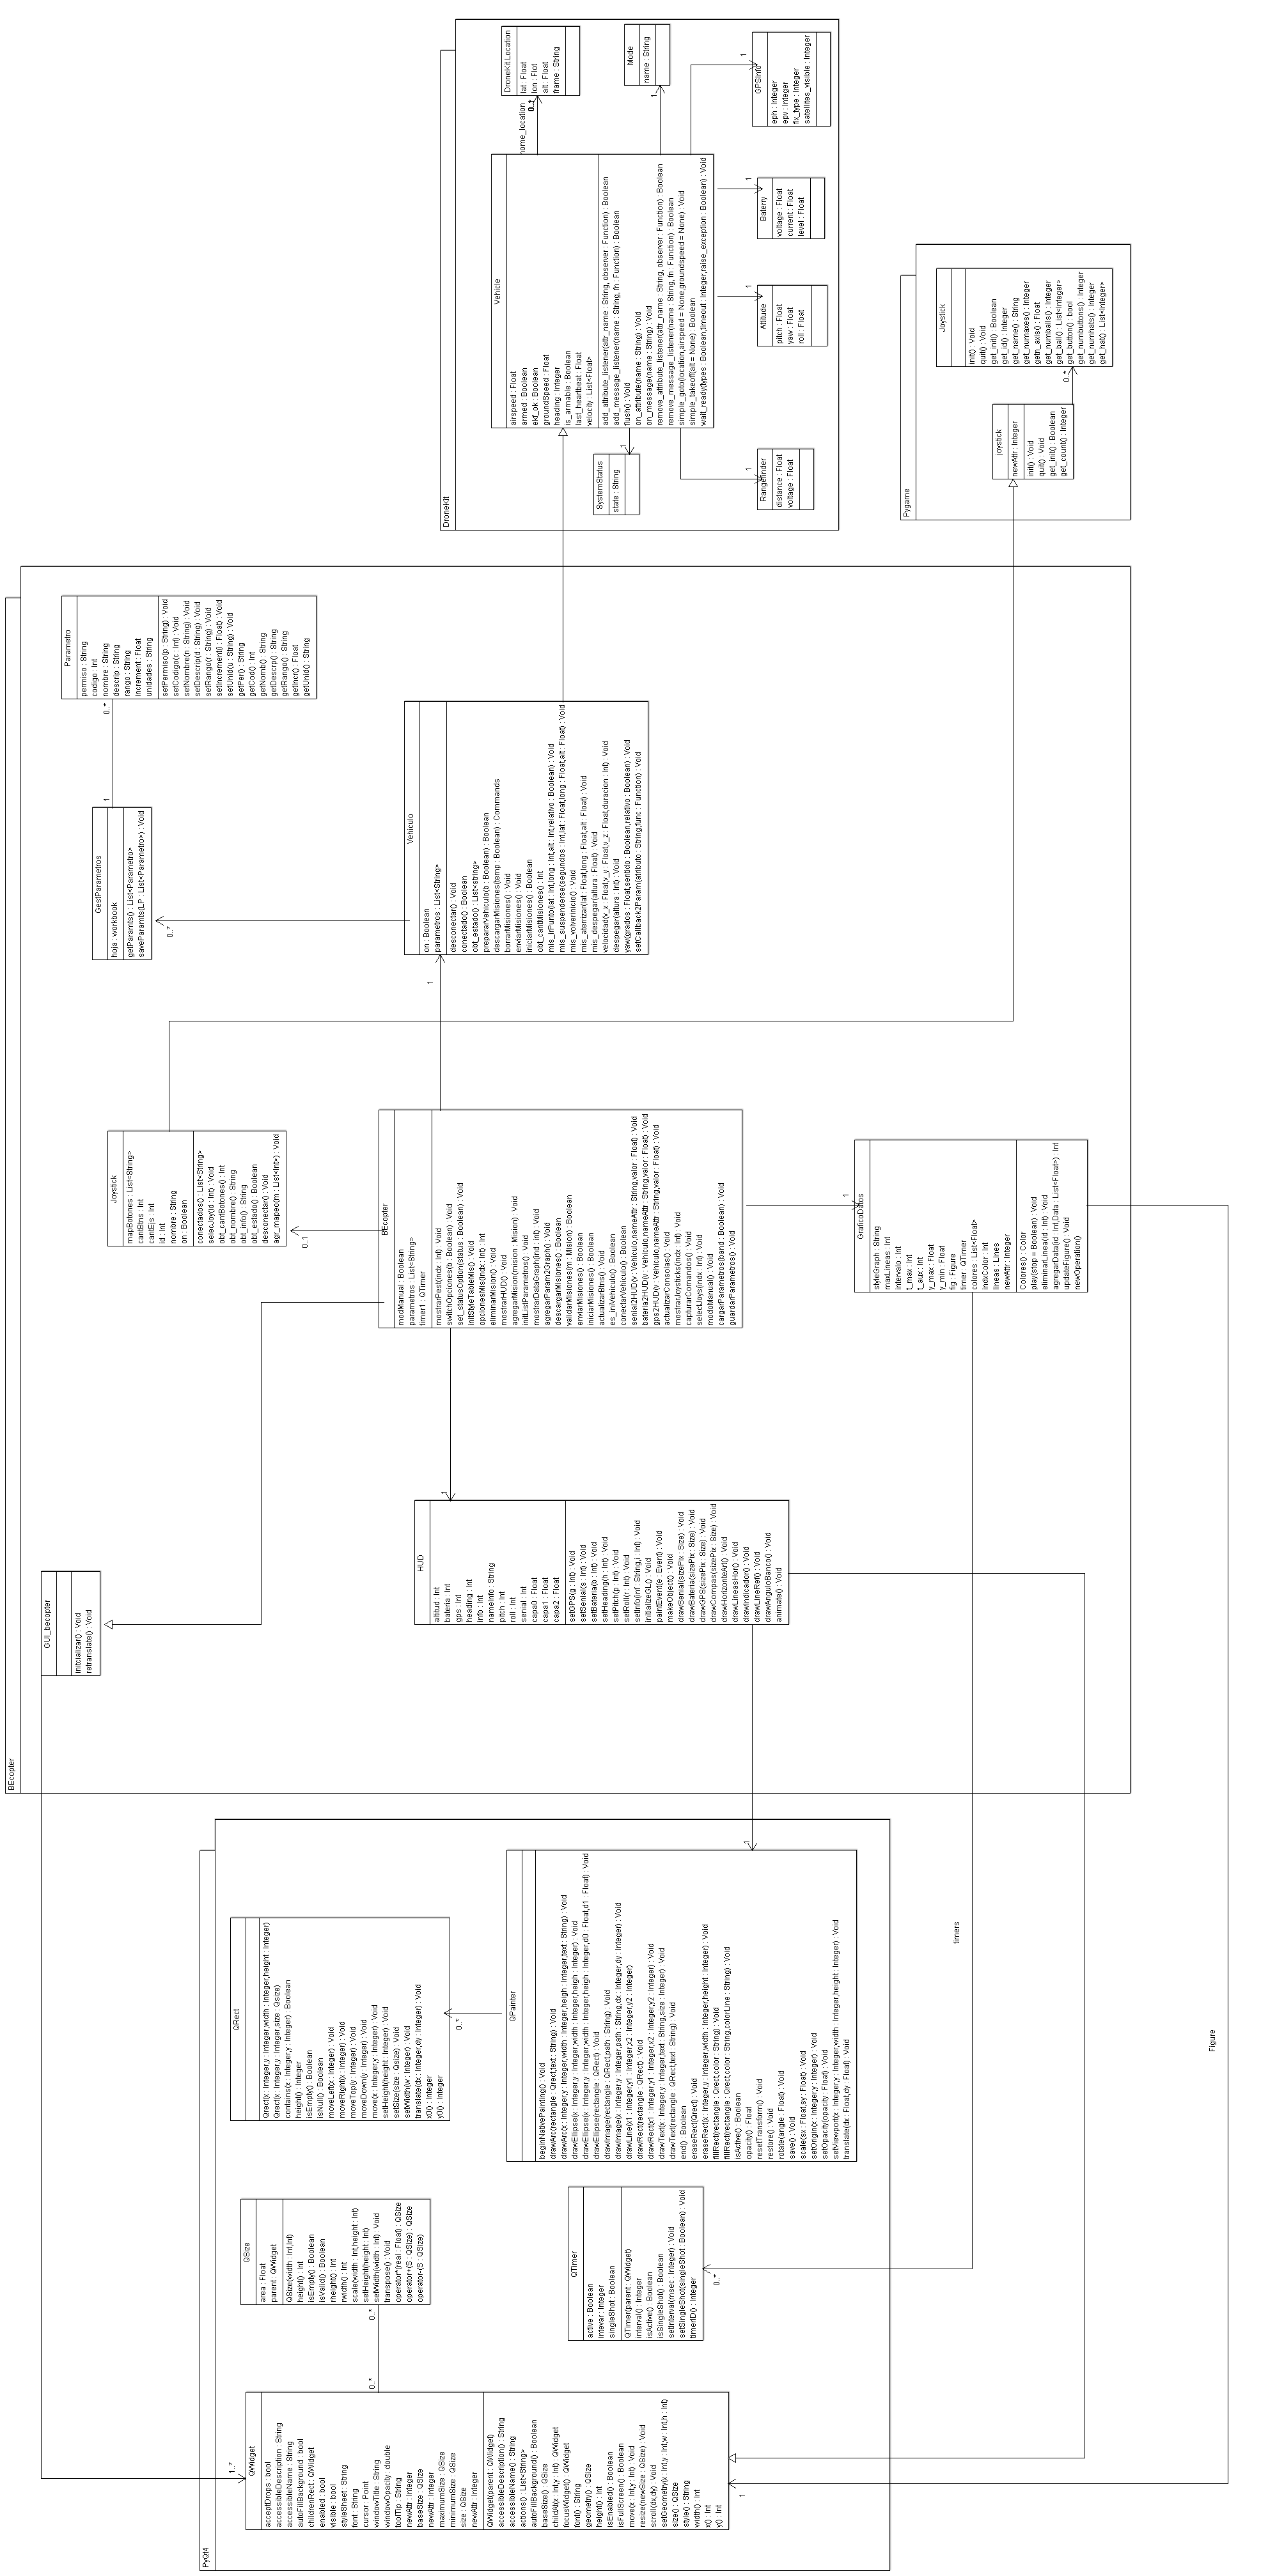
\includegraphics[width=\linewidth, height=0.93\textheight]{Apendice/Apendice_files/DC_BEcopter}
%			\caption{Diagrama de clases v2, perteneciente al proyecto BEcoper}
%			\label{fig:dcbecopter}
%		\end{figure}


% Variable local para emacs, para  que encuentre el fichero maestro de
% compilaci�n y funcionen mejor algunas teclas r�pidas de AucTeX
%%%
%%% Local Variables:
%%% mode: latex
%%% TeX-master: "../Tesis.tex"
%%% End:
